\documentclass{article}
%http://ctan.unixbrain.com/macros/latex/contrib/bytefield/
%\usepackage[margin=0.5in]{geometry}
%\usepackage{titling}
%\usepackage[compact]{titlesec}
\usepackage{fancyhdr} % custom headers
\usepackage{lastpage} % determine the last page for the footer
\usepackage{extramarks} % header footer
\usepackage{bytefield}
\usepackage{graphicx}
\usepackage{float}
\usepackage{url}
\usepackage[pdfborder={0 0 0}]{hyperref}
\usepackage[table]{xcolor}
\usepackage{microtype}
\usepackage[font=bf]{caption}
\usepackage{booktabs}
\usepackage{listings}

% margins
\topmargin=-0.45in
\evensidemargin=0in
\oddsidemargin=0in
\textwidth=6.5in
\textheight=9.0in
\headsep=0.25in

% line spacing
\linespread{1.1}

% empty line between paragraphs
\parskip = 0.5\baselineskip

% reduce spacing after figures
%\setlength{\belowcaptionskip}{-\baselineskip}

% setup header and footer
\pagestyle{fancy}
\lfoot{Sega Game Gear on a Chip}
\cfoot{}
\rfoot{Page\ \thepage\ of \protect\pageref{LastPage}}
\fancyhead[LE,RO]{\slshape \rightmark}
\fancyhead[LO,RE]{\slshape \leftmark}
\renewcommand\headrulewidth{0.4pt} % size of the header rule
\renewcommand\footrulewidth{0.4pt} % size of the footer rule

% remove indentation from paragraphs
\setlength\parindent{0pt}

% syntax highlighting
\definecolor{sh_comment}{rgb}{0.12, 0.38, 0.18}
\definecolor{sh_keyword}{rgb}{0.37, 0.08, 0.25}
\definecolor{sh_string}{rgb}{0.06, 0.10, 0.98}

\lstset{
    language=C,
    numbers=left,
    numberstyle=\tiny,
    frame=tb,
    showstringspaces=false,
    captionpos=b,
    stringstyle=\color{sh_string},
    keywordstyle = \color{sh_keyword}\bfseries,
    commentstyle=\color{sh_comment}\itshape,
    basicstyle=\small\sffamily,
    numbersep=-5pt,
    belowskip=-\parskip,
    aboveskip=\baselineskip
}

\title{
    \vspace{2in}
    \textbf{Sega Game Gear on a Chip}\\
    Design Report
    \vspace{3in}
}
\author{ Max Thrun | Samir Silbak}
\date{Fall 2012}

\begin{document}
\maketitle

\newpage
\tableofcontents
\newpage

\section{Abstract}
The objective of this project is to reimplement the hardware of the Sega Game
Gear (GG) in a Field Programmable Gate Array (FPGA). To do this each chip in
the system will be reimplemented in Verilog based on official and 3rd party
descriptions and specifications on how they operate. This document details the
design functionality and testing metrics that will be followed during the
implementation and execution of our project.

\section{System Overview}
The Sega Game Gear, released in 1991, was Sega's first attempt at a handheld
gaming console. It featured a Zilog Z80 clocked at 3.58MHz, 8KB of system RAM,
16KB of video ram, and a 160x144 pixel resolution screen.

\begin{figure}[H]
\centering
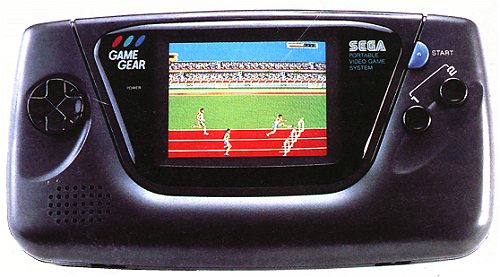
\includegraphics[scale=0.4]{../images/gamegear.png}
\caption{Sega Game Gear \protect\cite{gg}}
\label{fig:gg}
\end{figure}

The image below shows a picture of internal PCB of the Game Gear and it's major
components

\begin{table}[H]
    \centering
    \begin{tabular}{|c|l|c|l|}
        \hline
        1 & Zilog Z80 CPU           & 4 & 16K VRAM      \\ \hline
        2 & Video Display Processor & 5 & Sega BIOS ROM \\ \hline
        3 & 8K RAM                  & 6 & Controller IO \\
        \hline
    \end{tabular}
\end{table}

\newpage
\subsection{Functional Diagrams}
At a high level the Game Gear can be viewed simply as a system which takes
input from a game controller and produces video and audio as an output. This
description is shown in Figure~\ref{fig:external}.

\begin{figure}[H]
\centering
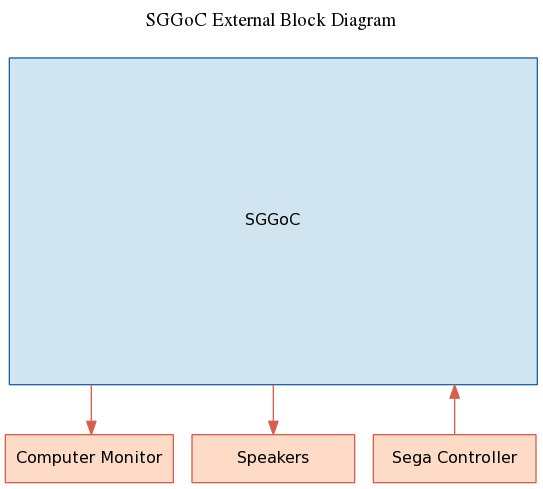
\includegraphics[scale=0.4]{../block_diagrams/block_diagram_external.png}
\caption{Black Box Diagram}
\label{fig:external}
\end{figure}

Internally the functionality can be easily modularized based on the actual
physical components found in the original Game Gear. Additional components will
be needed such as an IO controller and a memory management unit (MMU) to
account for the lack of tri-state buses in our design (explained later).
Figure~\ref{fig:internal} shows the interactions between the major functional
components in Sega Game Gear. The colored components are those which we
implemented in our project.

\begin{figure}[H]
\centering
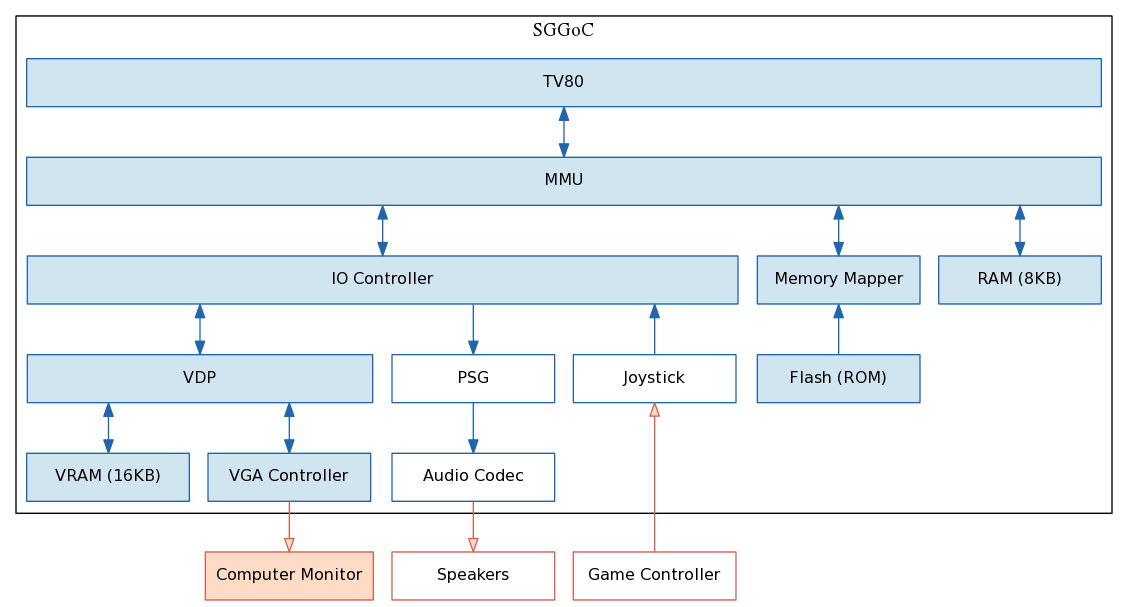
\includegraphics[scale=0.4]{../block_diagrams/block_diagram_internal_implemented.png}
\caption{Internal Functional Diagram}
\label{fig:internal}
\end{figure}

\newpage
\section{Cartridges and Memory Mapping}
The Z80 CPU only has 64KB of address space and 48KB of it is dedicated to the
game cartridge. A "mapper" is used to allow the use of larger ROMs (as well as
on-catridge RAM). Figure~\ref{fig:gg_cart} shows a standard GG cartridge and
Figure~\ref{fig:gg_cart_pcb} shows the internal PCB. The top chip is the Memory
Mapper and the bottom chip is the actual game ROM.

\begin{figure}[H]
    \centering
    \begin{minipage}[b]{0.3\linewidth}
        \centering
        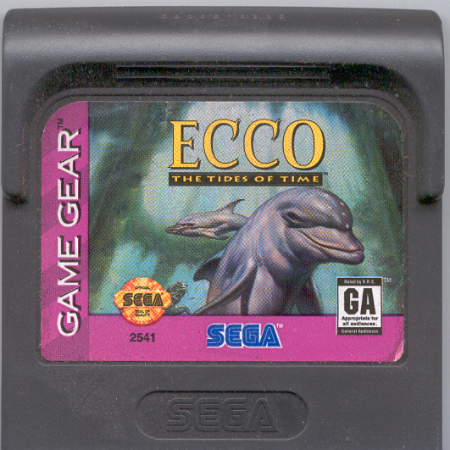
\includegraphics[height=2in]{../images/gg_cart.png}
        \caption{GG Cartridge \protect\cite{gg_cart}}
        \label{fig:gg_cart}
    \end{minipage}
    \hspace{1.5cm}
    \begin{minipage}[b]{0.3\linewidth}
        \centering
        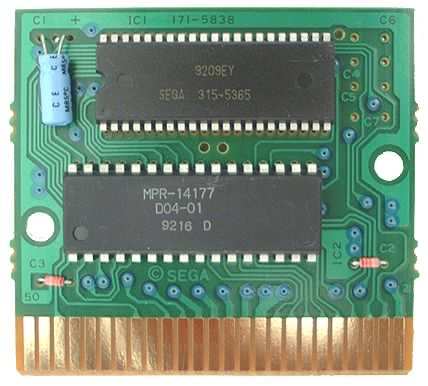
\includegraphics[height=2in]{../images/gg_cart_pcb.png}
        \caption{Cartridge PCB \protect\cite{gg_cart_pcb}}
        \label{fig:gg_cart_pcb}
    \end{minipage}
\end{figure}

\subsection{Sega Mapper}
There are several different mappers in existence but we will only focus on
implementing the "Sega Mapper" as it is the most popular.  The Sega mapper
defines 3 16KB slots in the Z80 memory map. Any 16KB bank of ROM can be mapped
into any of these 3 slots. The mapping is controlled by memory addresses
0xFFFC-0xFFFF.

\begin{table}[H]
    \centering
    \begin{tabular}{ccc}
        \toprule
        \textbf{Control Register} & \textbf{Slot} & \textbf{Maps to Z80 Address} \\
        \midrule
        \texttt{0xFFFC} & Control Bits & - \\
        \texttt{0xFFFD} & 0            & \texttt{0x0000-0x3FFF} \\
        \texttt{0xFFFE} & 1            & \texttt{0x4000-0x7FFF} \\
        \texttt{0xFFFF} & 2            & \texttt{0x8000-0xBFFF} \\
        \bottomrule
    \end{tabular}
    \caption{Mapper control registers \protect\cite{mapper}}
\end{table}

The ROM is viewed as an array of 16KB banks. The value written into the control
register determines which bank is selected for that slot.
Figure~\ref{fig:mapping_diagram} shows an example of how the address space gets
mapped to different ROM banks.

\begin{figure}[H]
\centering
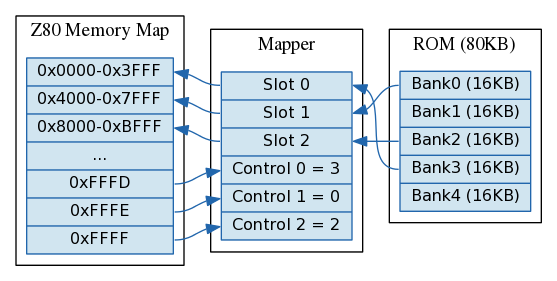
\includegraphics[height=1.5in]{../images/mapper.png}
\caption{Mapping Diagram}
\label{fig:mapping_diagram}
\end{figure}

\subsection{Cartridge Alternatives}
Since we are targeting a standard FPGA development board we cannot easily use
the actual game cartridge without some kind of hardware adaptor.  Additionally,
using the actual game cartridge would go against what we are trying to
accomplish with this project which is eliminating the need for any of the
original hardware. Lucky, virtually every Game Gear cartridge has been dumped
and are available online.  Unfortunately, the ROMs range in size all the way up
to 4MB and being that most affordable FPGAs do not have that much block RAM it
would be impossible for us to pack the ROM with the bitstream. A more ideal
solution would be to use a SD card which can be loaded with numerous ROM files
and then write a bootloader to select which one to play.  The complexity of
that strategy, however, is not worth the initial effort. A simpler solution
which would allow us to quickly start on the rest of the project is to load a
single ROM file onto the Flash chip that comes with our DE-1 development board.

\subsection{ROM Flasher}
The technical requirements of interfacing with the flash chip on our board are
outside the scope of our project and as such we will be using a core provided
by Altera \cite{flash_core} to simplify the process.
Figure~\ref{fig:flash_core} shows the black box diagram of the flash core
provided by Altera.

\begin{figure}[H]
\centering
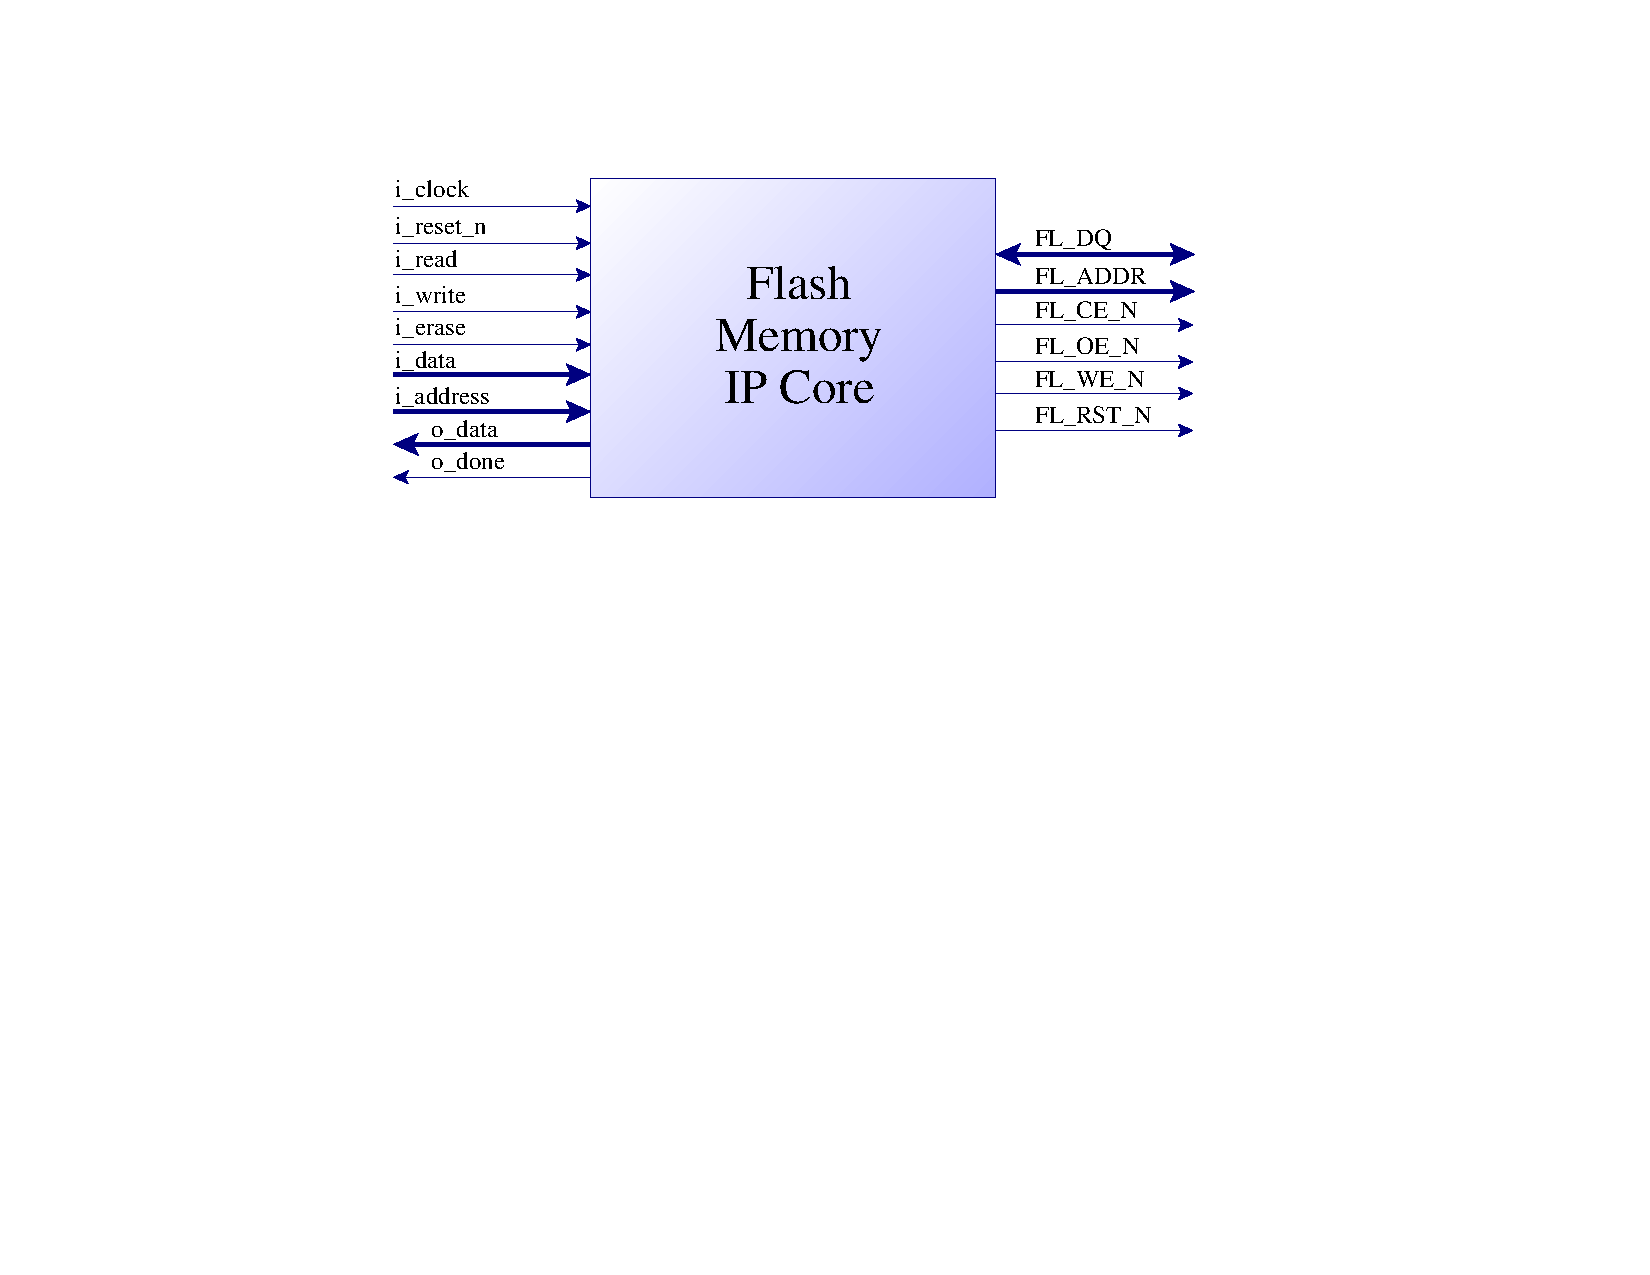
\includegraphics[scale=0.5]{../images/flash_core.pdf}
\caption{Altera Flash Core}
\label{fig:flash_core}
\end{figure}

A ``MemSend" project, completely separate from the GG project, will be used to
initially load a single ROM file into the flash chip.  On the computer a Python
program will read a ROM file byte by byte and send it to the FPGA over the
serial port. The FPGA will send back the byte it just recieved as an
acknowledgement. Another Python program will be used to read back and verify
that the flash contents match the ROM file. Figures~\ref{fig:rom_write}
and~\ref{fig:rom_read} illustrate the process of writing and reading a ROM to
and from the flash memory.

\begin{figure}[H]
    \centering
    \begin{minipage}[b]{0.45\linewidth}
        \centering
        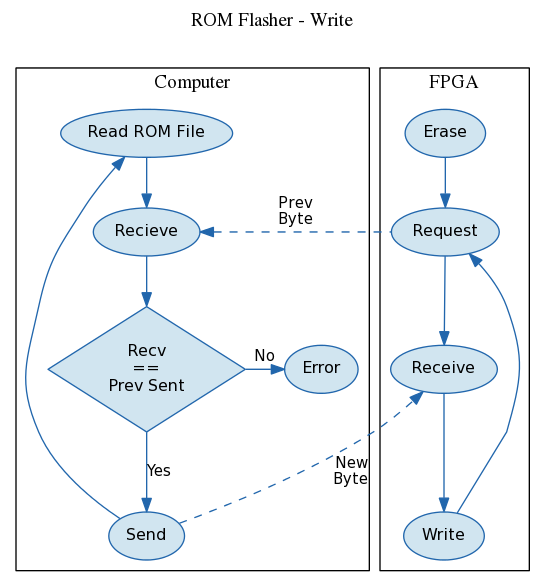
\includegraphics[width=\textwidth]{../../fpga/rom_flasher/doc/block_diagram_write.png}
        \caption{MemSend - Write}
        \label{fig:rom_write}
    \end{minipage}
    \hfill
    \begin{minipage}[b]{0.45\linewidth}
        \centering
        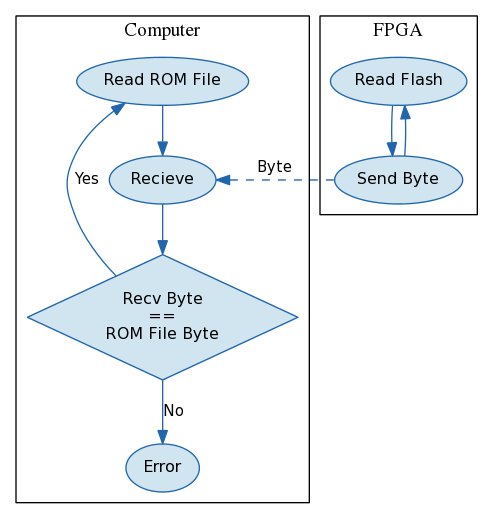
\includegraphics[width=\textwidth]{../../fpga/rom_flasher/doc/block_diagram_read.png}
        \caption{MemSend - Read}
        \label{fig:rom_read}
    \end{minipage}
\end{figure}

\section{Zilog Z80}
The Game Gear uses the classic Zilog Z80 CPU running at 3.58MHz as it's main
processor.  The re-implementation of the Z80 is completely outside the scope of
this project and as such we will be using the popular TV80 \cite{tv80} CPU
which is a proven, open source, implementation of the Z80 written in Verilog.
The interface of the TV80 exactly matches that of the original Z80, shown in
Figure~\ref{fig:z80}, with the only exception being the data bus. The original
Z80, as well as the whole Game Gear memory system, relies on tri-state buses
where as the TV80 has a separate bus for data in and data out.

\begin{figure}[H]
\centering
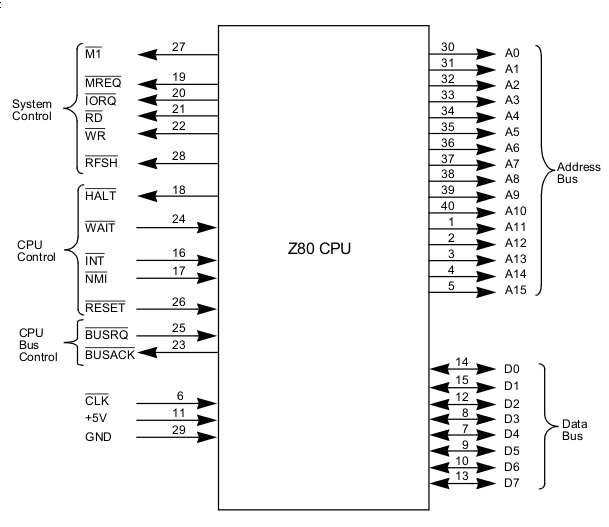
\includegraphics[scale=0.4]{../images/z80.png}
\caption{Zilog Z80}
\label{fig:z80}
\end{figure}

\section{Memory Management Unit (MMU)}
Since our design does not use tri-state buses we cannot simply connect the data
lines from each component together. Instead, we need to have some kind of
memory manager that can multiplex the data lines to whichever device the
address is pointing to according the system memory map. The full memory map for
the Game Gear is shown below

\begin{table}[H]
    \centering
    \begin{tabular}{ll}
        \toprule
        \textbf{Address} & \textbf{Device} \\
        \midrule
        \texttt{0x0000-0x03FF} & ROM (unpaged)                    \\
        \texttt{0x0400-0x3FFF} & ROM mapper slot 0                \\
        \texttt{0x4000-0x7FFF} & ROM mapper slot 1                \\
        \texttt{0x8000-0xBFFF} & ROM mapper slot 2 - OR - SaveRAM \\
        \texttt{0xC000-0xDFFF} & System RAM                       \\
        \texttt{0xE000-0xFFFF} & System RAM (mirror)              \\
        \texttt{0xFFFC}       & SaveRAM mapper control           \\
        \texttt{0xFFFD}       & Mapper slot 0 control            \\
        \texttt{0xFFFE}       & Mapper slot 1 control            \\
        \texttt{0xFFFF}       & Mapper slot 2 control            \\
        \bottomrule
    \end{tabular}
    \fontfamily{}\selectfont
    \caption{Z80 Memory Map \protect\cite{mem_map_table}}
\end{table}

Since the cartridge memory mapper handles the slot mapping itself we are really
only multiplexing between the cartridge and the system RAM.  The system RAM
happens to start at a nice edge being that \texttt{0xC000 = 0b1100000000000000}. To see
if we are accessing RAM we only need to check to see if bits 15 and 16 are
high. If so, we can simply use the 13 LSBs of the Z80 address as the index into
the RAM.  This method also accounts for the RAM mirror since the 13 LSBs repeat
starting at 0xE000.

\section{IO Controller}
\section{Video Display Processor (VDP)}

The Video Display Processor is a graphics chip which is derived from Texas
Instruments (TMS9918).

\subsection{Ports}

The VDP is accessed at the following Z80 I/O ports:

\begin{table}[H]
    \centering
    \begin{tabular}{c|p{3in}}
        \hline
        \hline
          \$7E & V counter (read) / SN76489 data (write)             \\
          \$7F & H counter (read) / SN76489 data (write, mirror)     \\
          \$BE & Data port (r/w)                                     \\
          \$BF & Control port (r/w)                                  \\
    \end{tabular}
\end{table}

The address decoding for the I/O ports is done with A7, A6 and A0 of the Z80
address bus, so the VDP locations are mirrored:

\begin{itemize}
    \item \$40 - 7F = Even locations are V counter/PSG, odd locations are H counter/PSG
    \item \$80 - BF = Even locations are data port, odd locations are control port.
\end{itemize}

%The H and V counters are described in the display timing section. The control
%and data ports are des

\subsection{Control port}

The VDP is programmed by sending a two-byte sequence to the control port. The
control port is used to define an offset into VRAM or CRAM for subsequent data
port I/O, and also to write to the internal VDP registers.
\\

There is a flag which is set after the first byte is sent and cleared when the
second byte is written. This insures the VDP to know which byte of the control
port is being received. Note that the flag is also cleared when the control
port is read, and when the data port is read or written. This is used to
initialize the flag to zero after it has been modified unpredictably, after an
interrupt routine has executed, for example.
\\

The VDP has two components that are used for accessing CRAM and VRAM:

\begin{itemize}
    \item address register
    \item code register
\end{itemize}

The address register is 14 bits in length and defines the address into VRAM
for reads and writes, and the address into CRAM for writes. The code register
is 2 bits in length and selects four different operations:

\begin{itemize}
    \item VRAM write
    \item VRAM read
    \item CRAM write
    \item VDP register write
\end{itemize}

The control port has the following format:

\begin{figure}[H]
    \centering
    \begin{bytefield}[bitwidth=2em, endianness=big]{8}
        \begin{rightwordgroup}{First Byte Written}
            \bitbox{1}{\tiny A07} & \bitbox{1}{\tiny A06} & \bitbox{1}{\tiny A05} & \bitbox{1}{\tiny A04} &
            \bitbox{1}{\tiny A03} & \bitbox{1}{\tiny A02} & \bitbox{1}{\tiny A01} & \bitbox{1}{\tiny A00}
        \end{rightwordgroup} \\
        \bitheader{0-7} \\
        \begin{rightwordgroup}{Second Byte Written}
            \bitbox{1}{\tiny CD1} & \bitbox{1}{\tiny CD0} & \bitbox{1}{\tiny A13} & \bitbox{1}{\tiny A12} &
            \bitbox{1}{\tiny A11} & \bitbox{1}{\tiny A10} & \bitbox{1}{\tiny A09} & \bitbox{1}{\tiny A08}
        \end{rightwordgroup} \\
        \bitheader{0-7}
    \end{bytefield}
    \caption{Caption Here}
    \label{fig:figure1234}
\end{figure}
Where,
\begin{table}[H]
    \centering
    \begin{tabular}{ll}
        \toprule
        \textbf{Bit} & \textbf{Definition} \\
        \midrule
        CDx & Code register     \\
        Axx & Address register  \\
        \bottomrule
    \end{tabular}
\end{table}

When the first byte is written, the lower 8 bits of the address register are
updated. When the second byte is written, the upper 6 bits of the address
register and the code register are updated, and the VDP may carry out
additional processing based on the value of the code register:

\begin{table}[H]
    \centering
    \begin{tabular}{cp{5in}}
        \toprule
        \textbf{Code} & \textbf{Actions Taken} \\
        \midrule
            0 & A byte of VRAM is read from the location defined by
                the address register and is stored in the read buffer.
                The address register is incremented by one. Writes to
                the data port go to VRAM.                                     \\
            1 & Writes to the data port go to VRAM                            \\
            2 & This value signifies a VDP register write, explained below.
                Writes to the data port go to VRAM.                           \\
            3 & Writes to the data port go to CRAM.                           \\
        \bottomrule
    \end{tabular}
\end{table}


When accessing CRAM, the upper bits of the address register are ignored as CRAM
is smaller than 16k (either 32 or 64 bytes depending on the VDP). The address
register will wrap when it exceeds \$3FFF.                                      \\

\textbf{VDP register write}                                                     \\

While the address and code register are updated like normal when a VDP register
write is done, the control port sent can be viewed as having a different format
to the programmer:

\begin{figure}[H]
    \centering
    \begin{bytefield}[bitwidth=2em, endianness=big]{8}
        \bitheader{0-7} \\
        \begin{rightwordgroup}{First Byte Written}
            \bitbox{1}{\tiny D07} & \bitbox{1}{\tiny D06} & \bitbox{1}{\tiny D05} & \bitbox{1}{\tiny D04} &
            \bitbox{1}{\tiny D03} & \bitbox{1}{\tiny D02} & \bitbox{1}{\tiny D01} & \bitbox{1}{\tiny D00}
        \end{rightwordgroup}\\
        \bitheader{0-7} \\
        \begin{rightwordgroup}{Second Byte Written}
            \bitbox{1}{\tiny 1}   & \bitbox{1}{\tiny 0}   & \bitbox{1}{\tiny X}   & \bitbox{1}{\tiny X} &
            \bitbox{1}{\tiny R03} & \bitbox{1}{\tiny R02} & \bitbox{1}{\tiny R01} & \bitbox{1}{\tiny R00}
        \end{rightwordgroup}
    \end{bytefield}
    \caption{Caption Here}
    \label{fig:figure1234}
\end{figure}

%\begin{table}[H]
%    \centering
%    \begin{tabular}{|l|l|}
%        \hline
%        MSB LSB                                                 \\ \hline
%        1   0   ?   ?   R03 R02 R01 R00 & Second byte written   \\ \hline
%        D07 D06 D05 D04 D03 D02 D01 D00 & First byte written    \\
%        \hline
%    \end{tabular}
%\end{table}

\begin{table}[H]
    \centering
    \begin{tabular}{l|l}
        \hline
        \hline
        RXX & VDP register number   \\
        DXX & VDP register data     \\
         X  & Ignored               \\
    \end{tabular}
\end{table}

The VDP selects a register using bits 3-0 of the second byte, and writes the
data from the first byte to the register in question. There are only 10
registers, values 11 through 15 have no effect when written to.
\\

\textbf{Data Port}

Depending on the code register, data written to the data port is sent to either
VRAM or CRAM. After each write, the address register is incremented by one, and
will wrap past \$3FFF.
\\

Reads from VRAM or CRAM are buffered. Every time the data port is read
(regardless of the code register) the contents of a buffer are returned. The
VDP will then read a byte from VRAM at the current address, and increment the
address register.  In this way data for the next data port read is ready with
no delay while the VDP reads VRAM. An additional quirk is that writing to the
data port will also load the buffer with the value written.

\subsection{Status Flags}

Reading the control port returns a byte containing status flags:

\begin{figure}[H]
    \centering
    \begin{bytefield}[bitwidth=2em, endianness=big]{8}
        \bitheader{0-7} \\
        \bitbox{1}{\tiny INT} & \bitbox{1}{\tiny OVR} & \bitbox{1}{\tiny COL} & \bitbox{1}{\tiny ---} &
        \bitbox{1}{\tiny ---} & \bitbox{1}{\tiny ---} & \bitbox{1}{\tiny ---} & \bitbox{1}{\tiny ---}
    \end{bytefield}
    \caption{Caption Here}
    \label{fig:figure1234}
\end{figure}

%\begin{table}[H]
%    \centering
%    \begin{tabular}{|l|}
%        \hline
%        MSB LSB                         \\ \hline
%        INT OVR COL --- --- --- --- --- \\
%        \hline
%    \end{tabular}
%\end{table}

\textbf{INT - Frame Interrupt Pending}

This flag is set on the first line after the end of the active display period.
It is cleared when the control port is read. (Please see the interrupts section
for more details).

\textbf{OVR - Sprite Overflow}

This flag is set if there are more than eight sprites that are positioned on a
single scanline. It is cleared when the control port is read.  (Please see the
sprites section for more information).

\textbf{COL - Sprite Collision}

This flag is set if an opaque pixel from any two sprites overlap. It is cleared
when the control port is read. (Please see the sprites section for more
information).

The remaining bits are not set by the VDP.

\subsection{Color RAM (CRAM)}

In Game Gear mode, CRAM has been expanded to 32 words or 64 bytes. Each word
defined a single color as shown below:

\begin{table}[H]
    \centering
    \begin{tabular}{l c l}
        - & = & Unused          \\
        R & = & Red pixels      \\
        G & = & Green pixels    \\
        B & = & Blue pixels     \\
    \end{tabular}
\end{table}

There are a total of 4096 (2\^{}12) possible colors that can be used, but only
32 colors can be shown at any given time.

The address register now wraps past address \$003F. Writing to an even CRAM
address causes the data written to be stored in a latch, and writing to an odd
CRAM address makes the VDP write the contents of the latch as well as the new
data from the CPU to the current CRAM entry. For example:

\begin{table}[H]
    \centering
    \fontfamily{pcr}\selectfont
    \begin{tabular}{p{1cm} p{1in} p{3.5in}}
        %\hline
        ld  &  hl, \$C000   & ; CRAM address \$0000                     \\
        rst &  10h          & ; Assume this functions sets VDP address  \\
        ld  &  a, \$FF      & ; Color data                              \\
        out &  (\$BE), a    & ; CRAM unchanged, latch = \$FF            \\
        ld  &  hl, \$C021   & ; CRAM address \$0021                     \\
        rst &  10h          & ; Set the address again                   \\
        ld  &  a, \$0F      & ; Color data                              \\
        out &  (\$BE), a    & ; CRAM word at \$0020 is now \$0FFF,
                                and the data at \$0000 is unchanged.    \\
        %\hline
    \end{tabular}
    \fontfamily{}\selectfont
    %\caption{
\end{table}

Therefore, writing single bytes to even CRAM addresses will not modify CRAM.
You could write multiple times to even addresses. This allows the same latched
color data to be written to multiple palette entries.

\subsection{Display Modes}

The TMS9918 has three bits which select different display modes called M1, M2,
and M3. Note that in the TMS9918 manual, there are only four modes documented:

\begin{table}[H]
    \centering
    \begin{tabular}{l c c l}
        Mode & 0 & - & Graphics I   \\
        Mode & 1 & - & Text         \\
        Mode & 2 & - & Graphics II  \\
        Mode & 3 & - & Multicolor   \\
    \end{tabular}
\end{table}

%\subsection{Tiles}
%\subsection{Layers}
%\subsection{Interrupts}
%\subsection{Display Timing}
\section{VGA Controller}

\newpage
\section{Testing}
\subsection{Custom Test ROMs}

In order to test the operation of the z80, and basic functionality of the VDP,
custom ROMs were developed. Using the Small Device C Compiler (SDCC)
\cite{SDCC} we are able to write programs that exercises various functionality
of the system.

We found SDCC extremely easy to setup and get working. The only thing we needed
to modify was the stack pointer location in the C Runtime file (crt0.s). The
default stack pointer location is set to \texttt{0xFFFF} but the top most RAM
address on the Game Gear is \texttt{0xDFFF}. Setting up IO is as easy as
specifying a special function register at a given IO port. An example showing
how to write data to the VDP data port (0xBE) is shown below.

\begin{lstlisting}[caption=VDP Data Write]
    __sfr __at (0xBE) vdp_data;
    int main() {
        vdp_data = 0x38;    // write 0x38 to VDP data port
        while (1) {}
        return 0;
    }
\end{lstlisting}

We ended up building a small GG library with the following functions:

\begin{lstlisting}[caption=Game Gear Library Functions]
    void vdp_write_control(uint8_t value);
    void vdp_write_data(uint8_t value);
    void vdp_set_register(uint8_t reg, uint8_t value);
    void vdp_set_vram_addr(uint16_t addr);
    void vdp_set_palette(uint8_t id, uint16_t color);
    void set_pattern_fill(uint16_t id, uint8_t color);
    void set_tile_to_pattern(uint8_t x, uint8_t y, uint16_t pattern);
    void delay(uint16_t x);
    void set_debug(uint8_t x);
\end{lstlisting}

With this library in place it is easy to to perform operations such as setting
up the color palette:

\begin{lstlisting}[caption=Color Palette Test ROM]
    #include <gg.h>
    int main() {
        // set register 1 bit 6 to enable display
        vdp_set_register(1, (1<<6));
        // set first color palette entry to gray
        vdp_set_palette(0, 0x0CCC);
        while (1) {}
        return 0;
    }
\end{lstlisting}

A few different test ROMs were developed to test drawing tiles and scrolling.
The ROMs were first run on an emulator to verify their functionality before
being loaded into flash on the FPGA board. The output of the `tiles' test ROM
is shown below:

\begin{figure}[H]
    \centering
    \begin{minipage}[H]{0.45\linewidth}
        \centering
        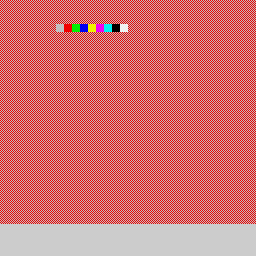
\includegraphics[width=\textwidth]{../images/tiles_screen.png}
        \caption{Tiles Screen}
        \label{fig:tiles_screen}
    \end{minipage}
    \hfill
    \begin{minipage}[H]{0.45\linewidth}
        \centering
        
\includegraphics[width=\textwidth]{../images/tiles_palette.png}
        \caption{Tiles Palette}
        \label{fig:tile_palette}
    \end{minipage}
\end{figure}


\subsection{VDP Background Generation}

In order to test the operation of the VDP background generator a separate test
project used which only consists of the background generator, VRAM, VGA timing
generator, and a UART interface.

Games are run using the open-source Osmose Sega Emulator \cite{osmose}. When
the game reaches a screen that we want to test on the FPGA we dump the VRAM and
CRAM using Osmoses built in debugger. We then use programs, written in C, that
read the VRAM dump and generate images of the color palette, all 512 background
tiles, and the final screen rendering.  These programs serve a dual purpose
allowing us to both confirm our understanding of how the background image is
generated and also that our VRAM dump is valid. The images below show example
output from these three programs.
\vfill
\begin{figure}[H]
    \centering
    \begin{minipage}[H]{0.45\linewidth}
        \centering
        
\includegraphics[width=\textwidth]{../images/palette.png}
        \caption{Color Palette}
        \label{fig:palette}
    \end{minipage}
    \hfill
    \begin{minipage}[H]{0.45\linewidth}
        \centering
        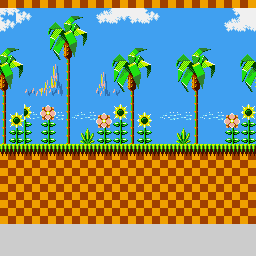
\includegraphics[width=\textwidth]{../images/screen.png}
        \caption{Complete Screen Render}
        \label{fig:screen}
    \end{minipage}
\end{figure}
\vfill
\begin{figure}[H]
    \centering
    \begin{minipage}[H]{0.8\linewidth}
        \centering
        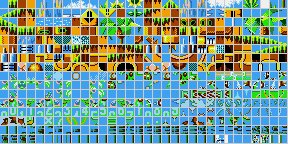
\includegraphics[width=\textwidth]{../images/tiles.png}
        \caption{All 512 Tiles}
        \label{fig:tiles}
    \end{minipage}
\end{figure}
\vfill
\newpage

After the VRAM dumps have been obtained they are loaded into the VRAM on the
FPGA via the same `MemSend' program introduced in the ROM section. The image
displayed on the monitor is then verified to ensure it matches both the
emulator and the output renderings of our C programs.

The testing strategy is executed as follows:
\begin{enumerate}
    \item Obtain VRAM dump from the Osmose emulator
        \begin{enumerate}
            \item Launch Osmose and open ROM file
                \begin{verbatim}$ ./Osmose-0-9-96-QT sonic.gg\end{verbatim}
            \item Set a scanline breakpoint in the debug console
                \begin{verbatim}Cmd: slbp 20\end{verbatim}
            \item Continue execution by entering `c' until the desired frame is reached.
            \item Dump the VRAM and CRAM
                \begin{verbatim}Cmd: davram 0\end{verbatim}
            \item Dump files are located at \texttt{/tmp/osmose.(vram,cram)}
        \end{enumerate}
    \item Verify dump integrity using C rendering programs
        \begin{enumerate}
            \item Run \texttt{screen}, located in \texttt{./tools/vdp\_render/}, on the dump files
            \item Ensure \texttt{screen.png} is generated
            \item Inspect \texttt{screen.png} pixel by pixel to ensure it matches the frame displayed in Osmose
            \item If image does not match another dump must be performed
            \item If image still does not match then debugging needs to be performed on the \texttt{screen} rendering program
        \end{enumerate}
    \item Transfer dump to FPGA VRAM via the `MemSend' tools
        \begin{enumerate}
            \item Flash the FPGA with the Video Display Processor test project located in \texttt{./fpga/vdp\_test/}
            \item Send a ROM file to the FPGA via the \texttt{send.py} program located in \texttt{./tools/mem\_send/}
            \item Ensure the \texttt{send.py} program completes without errors
        \end{enumerate}
    \item Verify that resulting image on screen
        \begin{enumerate}
            \item Inspect resulting image on monitor pixel by pixel and verify it matches both the original Osmose frame as well as the output from the C rendering programs
            \item If the image doe not match attempt to resend the rom
            \item If the image still does not match then debugging needs to be performed on the image rendering core.
        \end{enumerate}
\end{enumerate}

\newpage
\section{Standards}
\subsection{Verilog 2001}

The core of this project is built using the Verilog Hardware Description
Language defined by the IEEE standard 1364-2001 \cite{ieeeverilog}. This
standard describes the specifics of the Verilog language in regards to its
lexical structure, data types, expressions, hierarchical structures, and its
many other language features.  Fortunately for us, we can depends on the Altera
Quartus II compiler to ensure that all the requirements specified in the IEEE
standard are met. While the full standard is rather large we only need to
concern ourselves with a few sections, specifically the sections describing the
syntax (2, 3, 4, 6) and overall structure of how components are modeled (5, 9,
12, 14).

\subsection{GNU General Public Licensing Standard}

The GNU General Public License (GPL) \cite{gpl} is a standard, copyleft,
license for software and other works.  It guarantees end users the freedoms to
use, study, share, and modify the source code of the software so long as any
derivatives of the work is distributed under the same license. We felt that
this license was the best choice for our project given the fact that it is
primarily an academic pursuit and to be used, shared, and learned from.

\newpage
\begin{thebibliography}{9}
    \bibitem{gg} \url{http://mo5.com/musee-machines-gamegear.html}
    \bibitem{gg_cart} \url{http://www.magisterrex.com/prodimages/EccoDolphinGameGear-h450.png}
    \bibitem{gg_cart_pcb} \url{http://www.smspower.org/Development/SMSPagingChips}
    \bibitem{mapper} \url{http://www.smspower.org/Development/Mappers}
    \bibitem{flash_core} \url{ftp://ftp.altera.com/up/pub/flash/altera_up_flash_memory.zip}
    \bibitem{tv80} \url{http://opencores.org/project,tv80}
    \bibitem{mem_map_table} \url{http://code.google.com/p/bizhawk/source/browse/trunk/BizHawk.Emulation/Consoles/Sega/SMS/MemoryMap.Sega.cs}
    \bibitem{VDP} \url{http://www.smspower.org/uploads/Development/msvdp-20021112.txt?sid=c8bdf72dd28a0a34eeedf5f7742ca62a}
    \bibitem{osmose} \url{http://bcz.asterope.fr/osmose.htm}
    \bibitem{ieeeverilog} \url{http://ieeexplore.ieee.org/stamp/stamp.jsp?arnumber=00954909}
    \bibitem{gpl} \url{http://www.gnu.org/licenses/gpl.html}
    \bibitem{SDCC} \url{http://sdcc.sourceforge.net/}
\end{thebibliography}

\end{document}
